\section{Method}
\label{section:method}

This section describes the method with which the agents for rcssserver were defined and trained.

\subsection{Introduction}
The server \textit{ticks} every \(0.1\) seconds, wherewithin one command can be sent from each of the players and from the trainer. The program runs a loop in the background which sends a command from the trainer to the server continually (at each tick), requesting information about the state of the field at that time step. A state \(S_i \in \mathcal{S}\) where \(i \in \mathbb{N}\) contains the actual field state as well as the (possibly delayed) information thereabout which is known by the actors. Field-state information include the position and velocity of the ball as well as the speed, velocity and orientation of the players.

The players are represented as a set \(\mathcal{P}=\left\{p_1,\cdots,p_{12}\right\}\). A player \(p \in \mathcal{P}\) is a pair \((c, f)\) where \(c \in \mathcal{C} := \mathbb{N}^8\) is a vector representing the configuration of tweakable parameters for the player's actionable skills. (The parameters \(c_1,\cdots,c_8\in \mathcal{C}\) directly correspond to the in-program variables
\texttt{angle\_precision\_far}, \texttt{angle\_precision\_close}, \texttt{break\_distance}, \texttt{break\_amount}, \texttt{angle\_compensation\_far}, \texttt{angle\_compensation\_close}, \texttt{kick\_angle\_margin} and \texttt{kick\_distance\_power\_scale}.) \(f : \mathcal{S}\times \mathcal{C} \to \mathcal{S}\) is the the \textit{de facto} effect on the field state of an assigned action \(\mathfrak{a}\in\mathfrak{A}\), all of which return within one tick.

At each time step \(i\), a background process executes each player's ``configured'' task
\[
		%F := \left\{ f_p^c \,\middle|\, f_p^c = \lambda s.f_p(s, c), f_p = \pi_f(p), c = \pi_c(p), p \in\mathcal{P} \right\}
		F := \left\{ f_p^c \,\middle|\, f_p^c = \lambda s.f_p(s, c),\, (f_p, c) = p,\, p \in\mathcal{P} \right\}
\]
which sends commands from those players to the server, resulting in the next state
\begin{equation}
		S_{i} = \left\{
			\begin{array}{cl}
				S_I & : \ i = 0 \\
				\left(\underset{f_p^c\in F}\bigcirc f_p^c\right)(S_{i-1}) & : \ \text{otherwise}
			\end{array}
		\right. %\in \mathcal{S}
\end{equation}

where \(S_I\) is the initial configuration of the game field.
%and \(\mathfrak{U}\) is an unknown function representing collision handling and other unknown behaviours of the server simulation and program-server interface (such as the delayed field information). %RANDOMNESS MAKES THE SOLUTION-FINDING MODELING HARDER -- STATISTICS AND SUCH

\subsection{Behaviour tree}
The logic behind a player's action -- i.e., what commands are chosen for sendoff to the server in a given tick -- is defined by a behaviour tree generated by equation (2), the details whereof is stated in the following paragraphs.

Let \(\phi_\mathfrak{a}\in\Phi\subseteq\mathcal{S}\) be the set of all \textit{preconditional states} of an action \(\mathfrak{a}\in\mathfrak{A}\). A precondition of an action represents some statement about the set of all states \(\mathcal{S}\), such as ``a player cannot kick the ball unless it is near thereto'', or in other words, ``the set of all states where any agent \(p\in\mathcal{P}\) successfully kicks the ball \(\text{Kick}_p \subseteq \mathcal{S}\) is a subset to the set of all states where that player is near it \(\text{NearBall}_p \subseteq \mathcal{S}\), i.e., \(\text{Kick}_p \subseteq \text{NearBall}_p\)''.
%Let \(\pi(\phi)\in\mathfrak{A}\) be the action whose execution is supposed to bring about a set of states. \(\overset{\mathfrak{a}} \Pi : \underset{\Phi_\mathfrak{a}\in\Phi} \bigcup \Phi_\mathfrak{a} \to \mathfrak{A}\).

An action \(\mathfrak{a}\in\mathfrak{A}\) is either a symbol refering to some implemented function inside the program or it is a set of other actions in \(\mathfrak{A}\). \(\overset{\phi}\Pi : \mathfrak{A} \to \Phi\) is a map linking an action to its set of preconditional states. \(\overset{\mathfrak{a}}\Pi : \Phi \to \mathfrak{A}\) is a map linking preconditional states to the action whose execution is supposed to lead thereto.

A node of the behaviour tree is represented as a pair \(\langle \mathfrak{t}, \beta \rangle\) where \(\mathfrak{t}\in\mathfrak{T}\) is the \textit{type} of node -- sequence, selector, condition or action -- and \(\beta\) is a vector (from left to right) of the nodes' children. The function \(\text{BT}:\Phi\cup\mathfrak{A} \to \mathscr{B}\) (where \(\mathscr{B}\) is the set of all behaviour trees) generates the appropriate behaviour tree for an action given its definition and preconditions. The definition of \(\text{BT}(\omega)\) is given in equation (2).

%\onecolumn
%\begin{equation}
%		\text{BT}(\omega) := \left\{
%			\begin{array}{cl}
%					\left\langle \boxed{\to}, \left(\text{BT}\left(\overset{\mathfrak{\phi}} \Pi (\omega)\right), \text{BT}(\omega')\right) \right\rangle \ \text{for any}\  \omega' \in \omega & : \ \text{Set}(\omega') \wedge \omega\in\mathfrak{A} \\
%					\left\langle \boxed{?}, \left(\omega,\text{BT}\left(\overset{\mathfrak{a}} \Pi (\omega)\right)\right) \right\rangle & : \ \omega\in\Phi \\
%					\left\langle \omega, () \right\rangle & : \ \text{otherwise}
%			\end{array}
%		\right.
%\end{equation}
%\twocolumn
\begin{figure*}[h!]
	\centering
    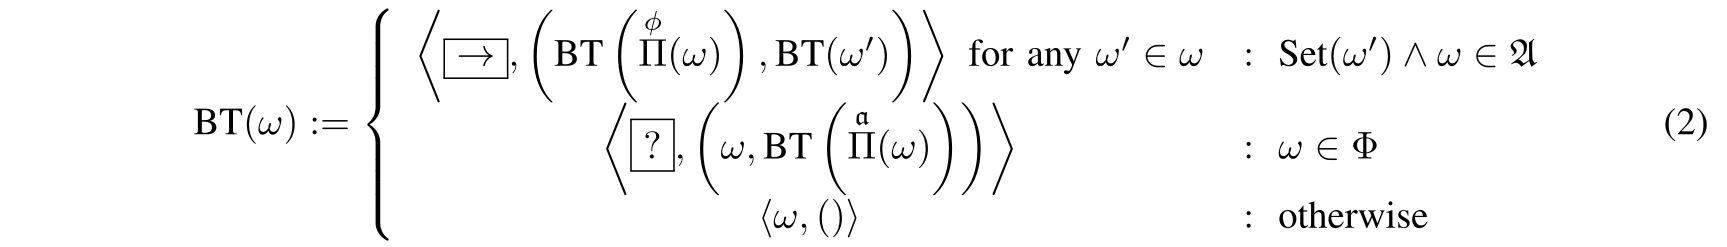
\includegraphics[width=\textwidth]{equation2.png}
    \label{fig:fullbredd}
\end{figure*}

In this way, the behaviour tree will always choose to execute the actions which lead to any of the states in the desired set\footnote{The proof hereof is omitted.}. The behaviour tree generated by the action ``move ball to location'' is shown in figure 2.

\begin{figure*}[tbp]
\centering
\begin{forest}
  for tree={draw,
			align=center
		},
		[Ø
			%[\(\to\)
				[?
					[\textit{Ball near}\\\textit{location?}, rounded corners
]
					[\(\to\)
						[?
							[\textit{Player near}\\\textit{ball?}, rounded corners
							]
							[\(\to\)
								[?
									[\textit{Player at}\\\textit{breaking}\\\textit{distance?}, rounded corners
]
									[\(\to\)
										[?
											[\textit{Player facing}\\\textit{target (far)?}, rounded corners
]
											[\texttt{alignFar()}]
										]
										[\texttt{goTowardFar()}]
									]
								]
								[\(\to\)
									[?
										[\textit{Player facing}\\\textit{target (close)?}, rounded corners
]
										[\texttt{alignClose()}]
									]
									[\texttt{goTowardClose()}]
								]
							]
						]
						[\(\to\)
							[?
								[\textit{Player}\\\textit{aligned}\\\textit{to kick?}, rounded corners
]
								[\texttt{alignKick()}]
							]
							[\texttt{kickBall()}]
						]
					]
				]
			%]
		]
\end{forest}
	\caption{Behaviour tree generated by equation (2) for the action ``move ball to location''}
\label{fig:gene}
\end{figure*}

\subsection{Genetic algorithm}
A monoid \(M_f:=\left(\langle \right\{ f \left\} \rangle,\circ\right)\) is compositionally generated by the map \(f\), corresponding to some action \(\mathfrak{a}\in\mathfrak{A}\), the ``completion'' set of which is denoted \(\xi_\mathfrak{a}\subseteq\mathcal{S}\). The set \(V_\mathfrak{a} := \left\{ c\in\mathcal{C} \,\middle|\, \exists N\in\mathbb{N},\, \overset{N}{\underset{n=1}\bigcirc} f^c \in \mathcal{S} \to \xi_\mathfrak{a} \right\}\) contains every configuration that can always provide a solution to \(\mathfrak{a}\).

%The set of all solutions to an action given a configuration, then, is defined as
%\[
%		\mathscr{S}^c_\mathcal{\xi_\mathfrak{a}} = \left\{ n\in\mathbb{N} \,\middle|\, \mathcal{G}\subseteq M\wedge\overset{1}{\underset{i=|s^c|}\bigcirc} s^c_i \in \mathcal{G} \right\}
%\]

%We want to approximate the set \(C\subseteq\mathcal{C}\) such that \( \forall \mathfrak{a}\in\mathfrak{A},\, V_\mathfrak{a}\subseteq\mathcal{C} \) and \(C'\subseteq\mathcal{C} \Rightarrow \forall \mathfrak{a} \left( \text{min} \left( |s| V_\mathfrak{a} \right) \right)\)
Let \(\mathscr{L}^c_\mathfrak{a}\) denote the \textit{length} of the shortest solution for a given task \(\mathfrak{a}\) and configuration \(c\in V_\mathfrak{a}\). To approximate a configuration \(c\in\mathcal{C}\) such that \( \forall \mathfrak{a}\in\mathfrak{A},\, c\in V_\mathfrak{a} \) and \(c'\in\mathcal{C} \Rightarrow \forall \mathfrak{a},\, \mathscr{L}^{c'}_\mathfrak{a} \ge \mathscr{L}^{c}_\mathfrak{a}\), \(\mathfrak{a}\) and \(\xi_\mathfrak{a}\) are constrained.

Since the action ``move ball to location'' is affected by all variables in the vector \(c\), optimizing it will optimize all values in the configuration. Thus, \(\mathfrak{a}\) equals this action hereafter with the completion set \(\xi_\mathfrak{a}\) defined as \(L(x,y,m) = \left\{ S \in \mathcal{S} \,\middle|\, \sqrt{ \left(S_{\text{ball}_x} - x\right)^2 + \left(S_{\text{ball}_y} - y\right)^2 } \le m \right\}\).

The genetic algorithm considers \(\mathscr{L}^{c}_\mathfrak{a}\) -- the \textit{loss function} -- for all \(c\in G_i\), where \(G_i\in\mathcal{C}^{12}\) denotes the generation \(i\).

The training ensures \(\)
